\newpage
\subsection{Actividad 15}
Diseñar un controlador analógico tipo PID (PD, PI, PID) para el
sistema servomotor de velocidad por el \textsc{método de Rivera-Morari} y de
síntesis directa y realizar su discretizacion con $T=0.05$ aplicando el
método de emparejaiento polos-ceros y graficar la respuesta escalón
unitaria del sistema de control en bucle cerrado del servomotor de
velocidad a través de la herramienta \textsc{rltool}.

\begin{tcolorbox}[sharp corners, colframe=bluebox, title= Controlador
  síntesis directa, breakable=unlimited]
Primero comprobamos si se puede controlar a través de este método. Para ello, 
el sistema debe ser estable en bucle abierto.

 $>>>$ step(Gvelocidad)
  \mkanscode{
\begin{figure}[H]
  \centering
  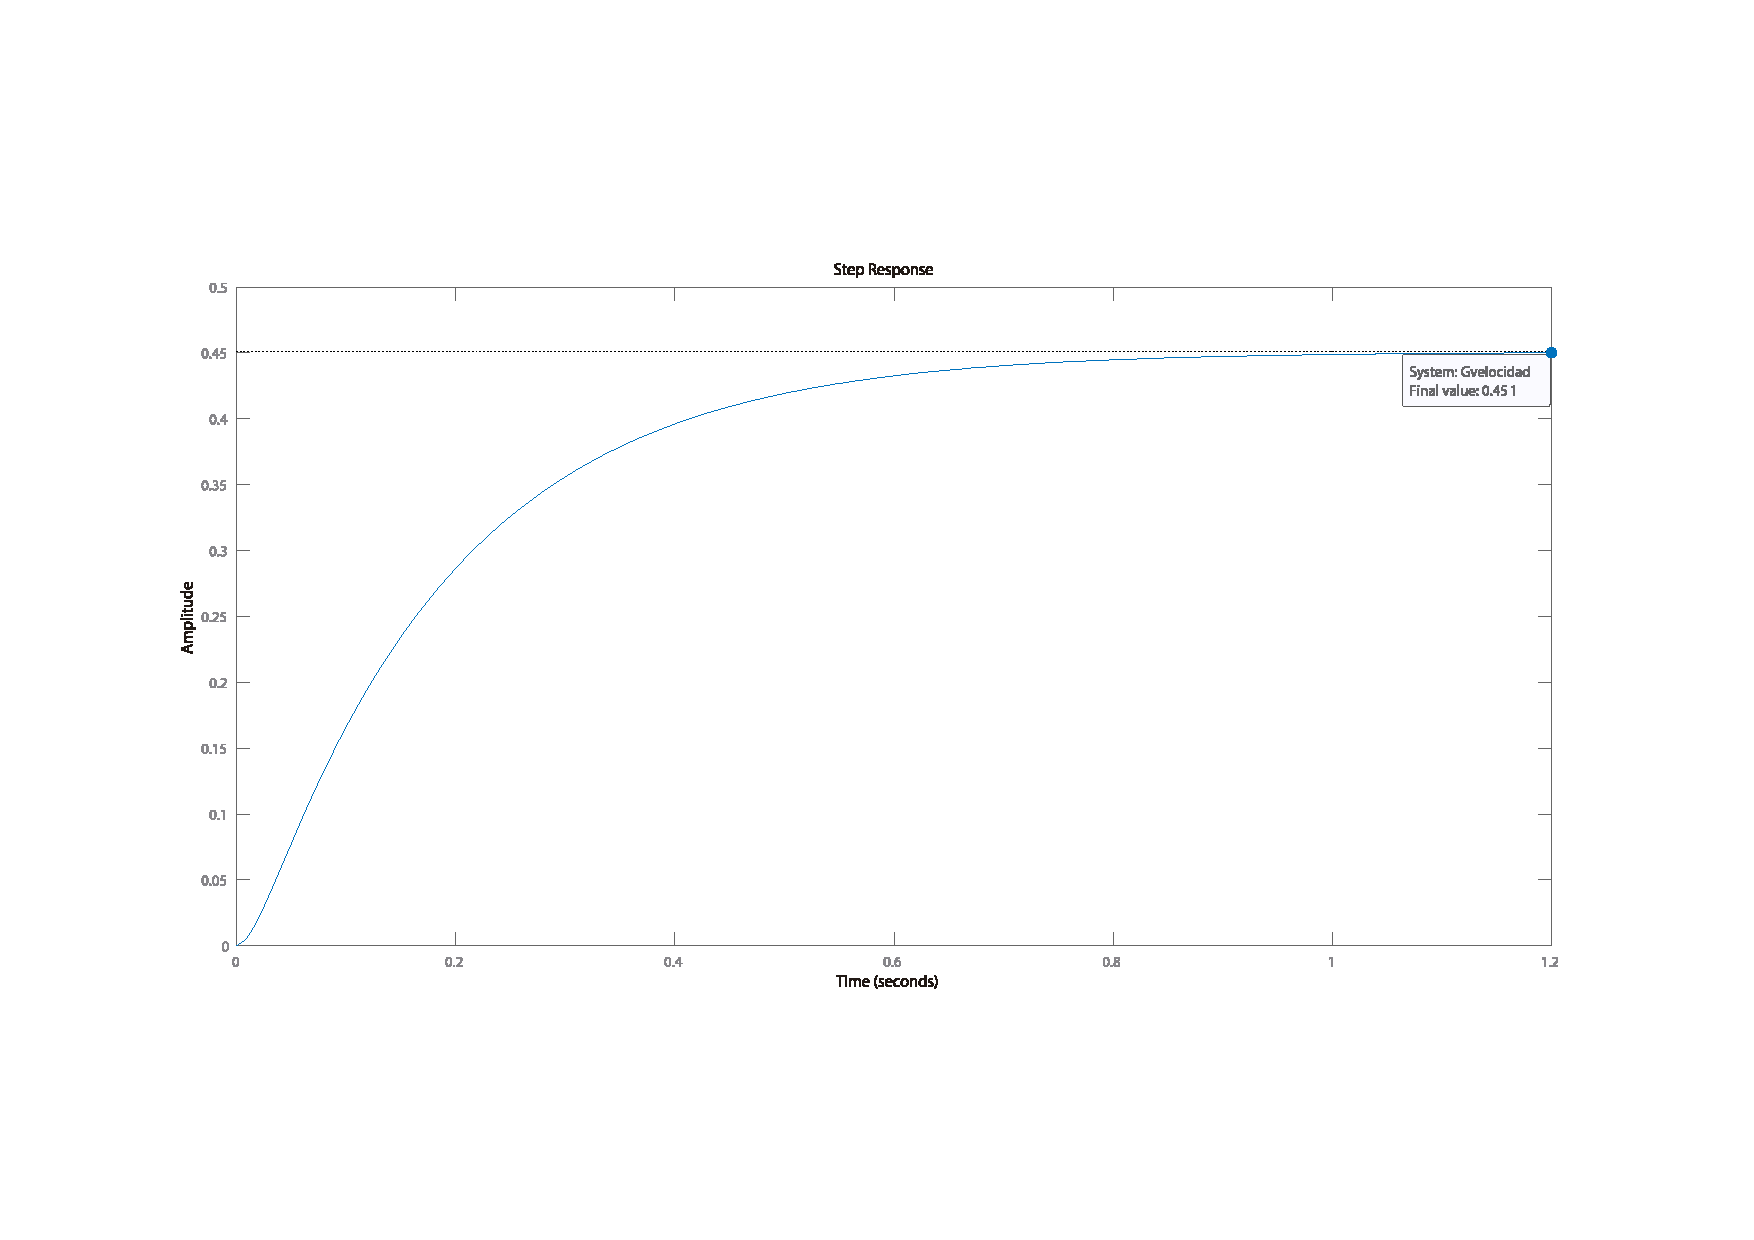
\includegraphics[clip, trim=4cm 4.5cm 3cm 4.5cm,scale=0.48]{images/figura 20.pdf}
  % izquierda,abajo,derecha,arriba
  \caption{Respuesta del sistema abierto frente a un escalón.}
    \label{fig:figura 20}
\end{figure}
  }
Según la respuesta del sistema en bucle abierto, es estable por lo que 
se puede aplicar. Nuestra planta es una planta de segundo orden
sobreamortiguada.

Calculamos los polos del sistema en bucle abierto

$>>>$ [polo1,polo2]= pole(Gvelocidad);

Se calculan los parámetros:\\
$k$ Es el valor final en bucle abierto, por lo tanto, $k = 0.451$.\\
$>>>$ tau\_1 =  1/63.5465\\
$>>>$ tau\_2 =  1/5.4951\\

Nuestra lamda debe ser mayor que $0.2*\tau_{max} = 0.2 *\tau_2 = 5.4951$.\\
Vamos a tomar\\
$>>>$ lambda = 6\\
$>>>$ k = 0.451;kp=(tau\_1+tau\_2)/(k*lamda);\\
$>>>$ ti = tau\_1 + tau\_2;\\
$>>>$ td = (tau\_1*tau\_2)/(tau\_1+tau\_2);\\
$>>>$ PID = pidstd(kp,ti,td)\\

  \vspace*{0.5em}
  \begin{tcolorbox}[sharp corners, colback = white]
    \color{gray}
\begin{verbatim}

PID =
 
             1      1          
  Kp * (1 + ---- * --- + Td * s)
             Ti     s          

  with Kp = 0.0731, Ti = 0.198, Td = 0.0145
 
Continuous-time PID controller in standard form
\end{verbatim}
  \end{tcolorbox}%
  \vspace*{0.5em}

$>>>$ C = c2d(PID,0.05,'matched')

    \vspace*{0.5em}
  \begin{tcolorbox}[sharp corners, colback = white]
    \color{gray}
\begin{verbatim}
C =
 
             1       Ts            z-1 
  Kp * (1 + ---- * ------ + Td * ------)
             Ti      z-1           Ts  

  with Kp = 0.0961, Ti = 0.26, Td = 0.0417, Ts = 0.05
 
Sample time: 0.05 seconds
Discrete-time PID controller in standard form
\end{verbatim}
  \end{tcolorbox}%
  $>>>$  step(kw*feedback(Gvelocidadz*C,kw))
      \vspace*{0.5em}
    \mkanscode{
\begin{figure}[H]
  \centering
  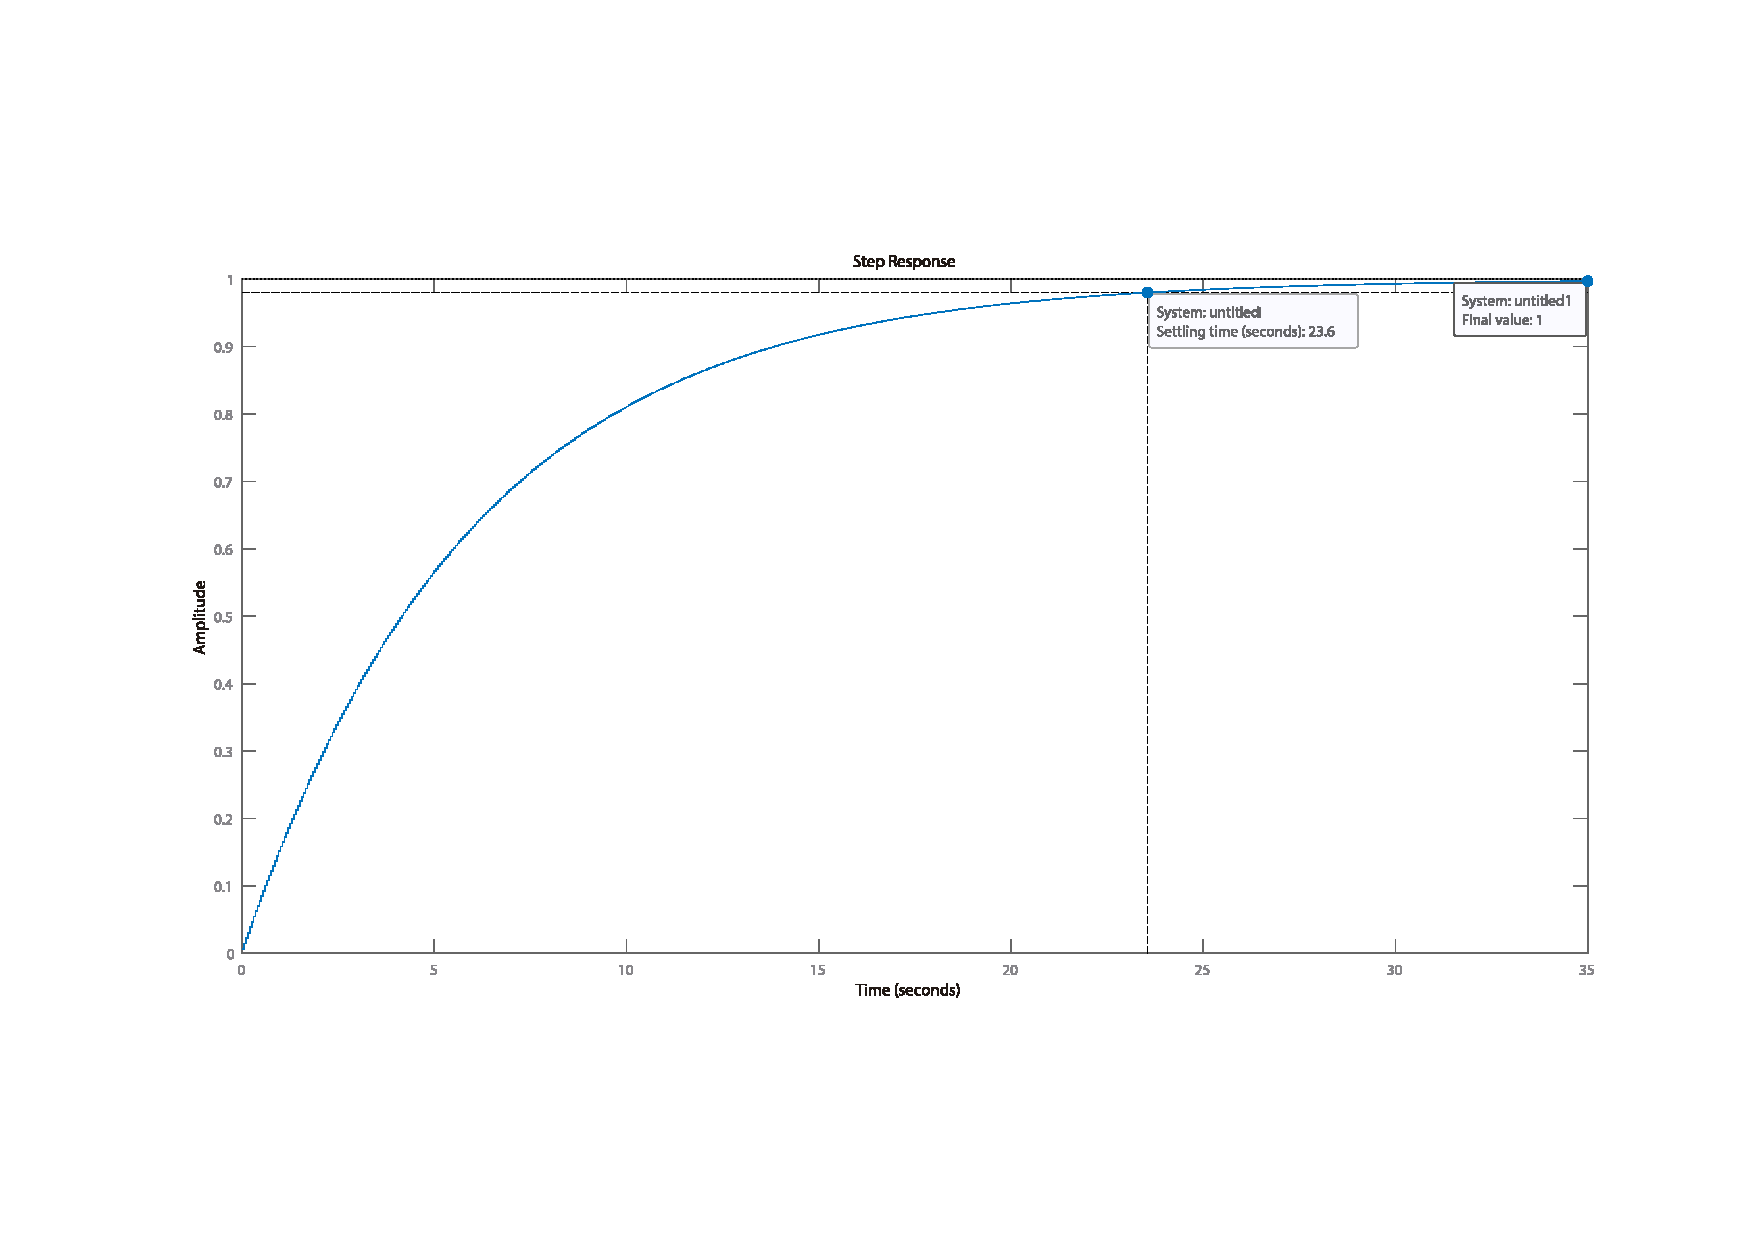
\includegraphics[clip, trim=2.5cm 3.5cm 2.8cm 4.5cm,scale=0.48]{images/figura 21.pdf}
  % izquierda,abajo,derecha,arriba
  \caption{Respuesta del sistema cerrado frente a un escalón.}
    \label{fig:figura 21}
\end{figure}
  }
\end{tcolorbox}%

\begin{tcolorbox}[sharp corners, colframe=bluebox, title= Controlador Rivera-Morari, breakable=unlimited]
Primero comprobamos si se puede controlar a través de este método. Para ello, 
el sistema debe ser estable en bucle abierto.

 $>>>$ step(Gvelocidad)
  \mkanscode{
\begin{figure}[H]
  \centering
  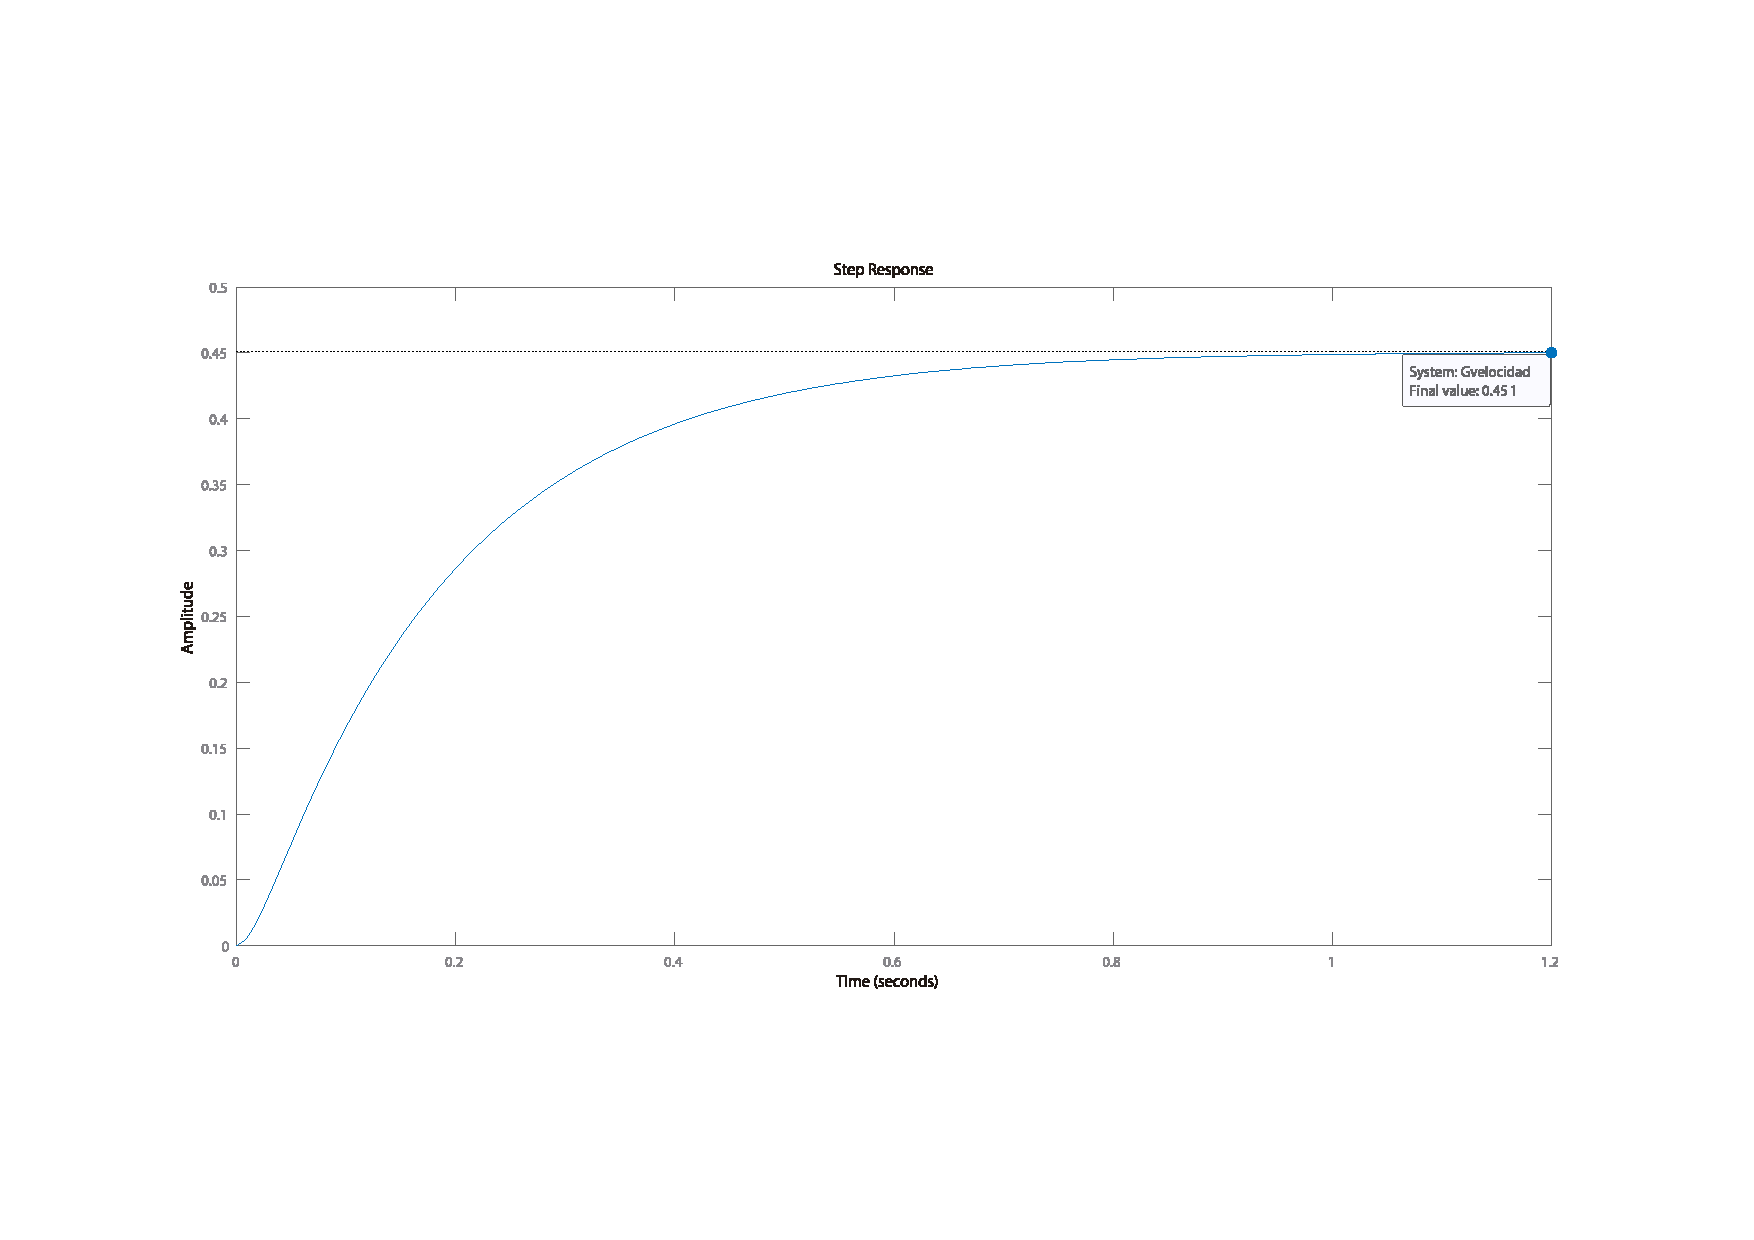
\includegraphics[clip, trim=4cm 4.5cm 3cm 4.5cm,scale=0.48]{images/figura 20.pdf}
  % izquierda,abajo,derecha,arriba
  \caption{Respuesta del sistema abierto frente a un escalón.}
    \label{fig:figura 20}
\end{figure}
}
A partir de la respuesta de nuestro sistema obtenemos:\\
$>>>$ k = 0.451\\
$>>>$ t632=0.119;t283=0.0773;\\

Obtenemos los parámetros para calcular nuestro PID:\\
$>>>$ d=3*(t632-t283)/2;tau=t632-d;\\
Es recomendable que $\lambda > 0.2*\tau=0.0113$\\
Y que cumpla que $\lambda/d > 1.7$, es decir, $\lambda > d*1.7 = 0.1063$\\
Elegiremos nuestro lamda\\
$>>>$ lamda = 1;\\
Llendo a la tabla de PI\\
$>>>$ kp = tau/(k*lamda);ti=tau;

Nuestro PI es:\\
$>>>$ PI = pidstd(kp,ti)
  \vspace*{0.5em}
  \begin{tcolorbox}[sharp corners, colback = white]
    \color{gray}
\begin{verbatim}
PI =
 
             1      1 
  Kp * (1 + ---- * ---)
             Ti     s 

  with Kp = 0.125, Ti = 0.0565
 
Continuous-time PI controller in standard form
\end{verbatim}
  \end{tcolorbox}%
  \vspace*{0.5em}

$>>>$ C = c2d(PID,0.05,'matched')

    \vspace*{0.5em}
  \begin{tcolorbox}[sharp corners, colback = white]
    \color{gray}
\begin{verbatim}
C =
 
             1       Ts  
  Kp * (1 + ---- * ------)
             Ti      z-1 

  with Kp = 0.189, Ti = 0.0851, Ts = 0.05
 
Sample time: 0.05 seconds
Discrete-time PI controller in standard form

\end{verbatim}
  \end{tcolorbox}%
  $>>>$  step(kw*feedback(Gvelocidadz*C,kw))
      \vspace*{0.5em}
    \mkanscode{
\begin{figure}[H]
  \centering
  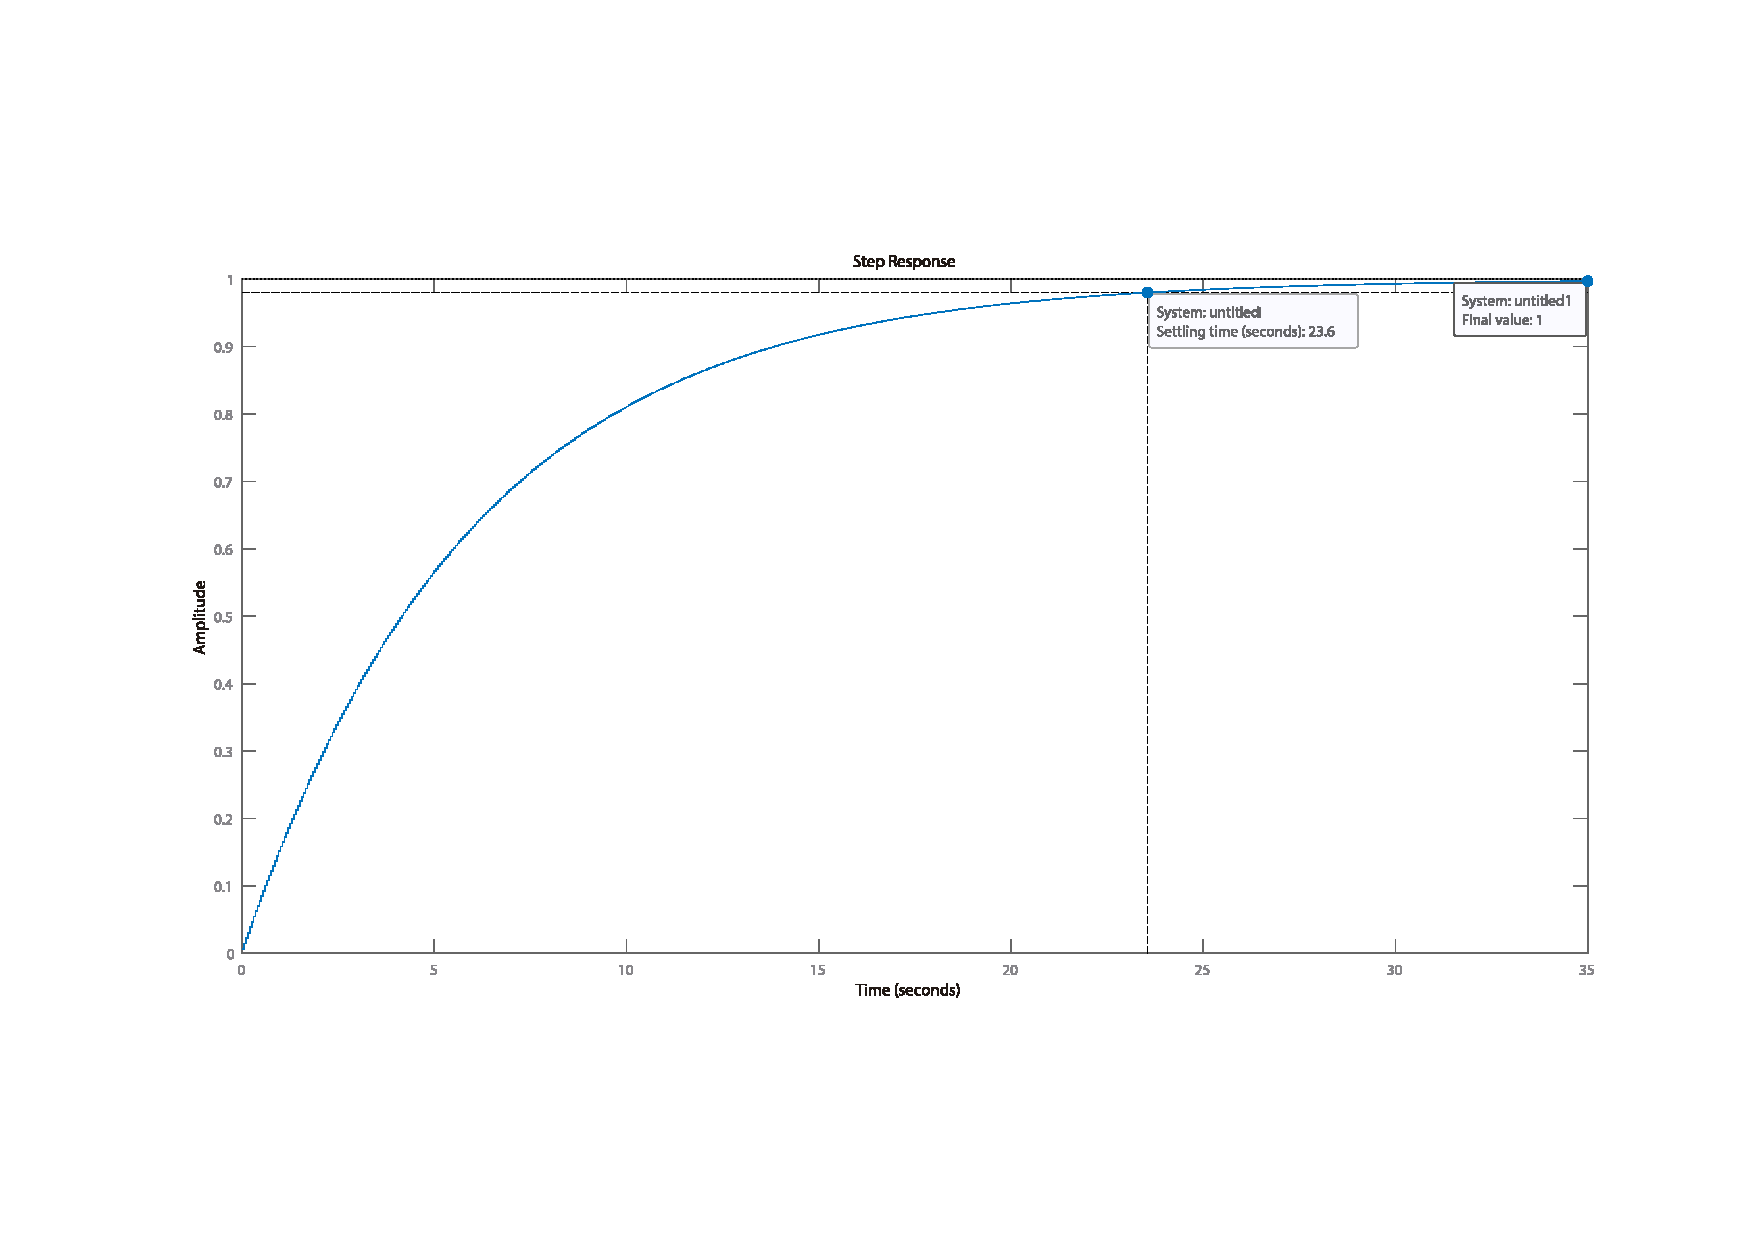
\includegraphics[clip, trim=2.5cm 3.5cm 2.5cm 4.5cm,scale=0.48]{images/figura 21.pdf}
  % izquierda,abajo,derecha,arriba
  \caption{Respuesta del sistema cerrado frente a un escalón.}
    \label{fig:figura 21}
\end{figure}
  }
  \end{tcolorbox}%